\section{Headless-AD}
\label{section:headless_ad}

\begin{figure}[!t]
    \vskip 0.2in
    \centering
    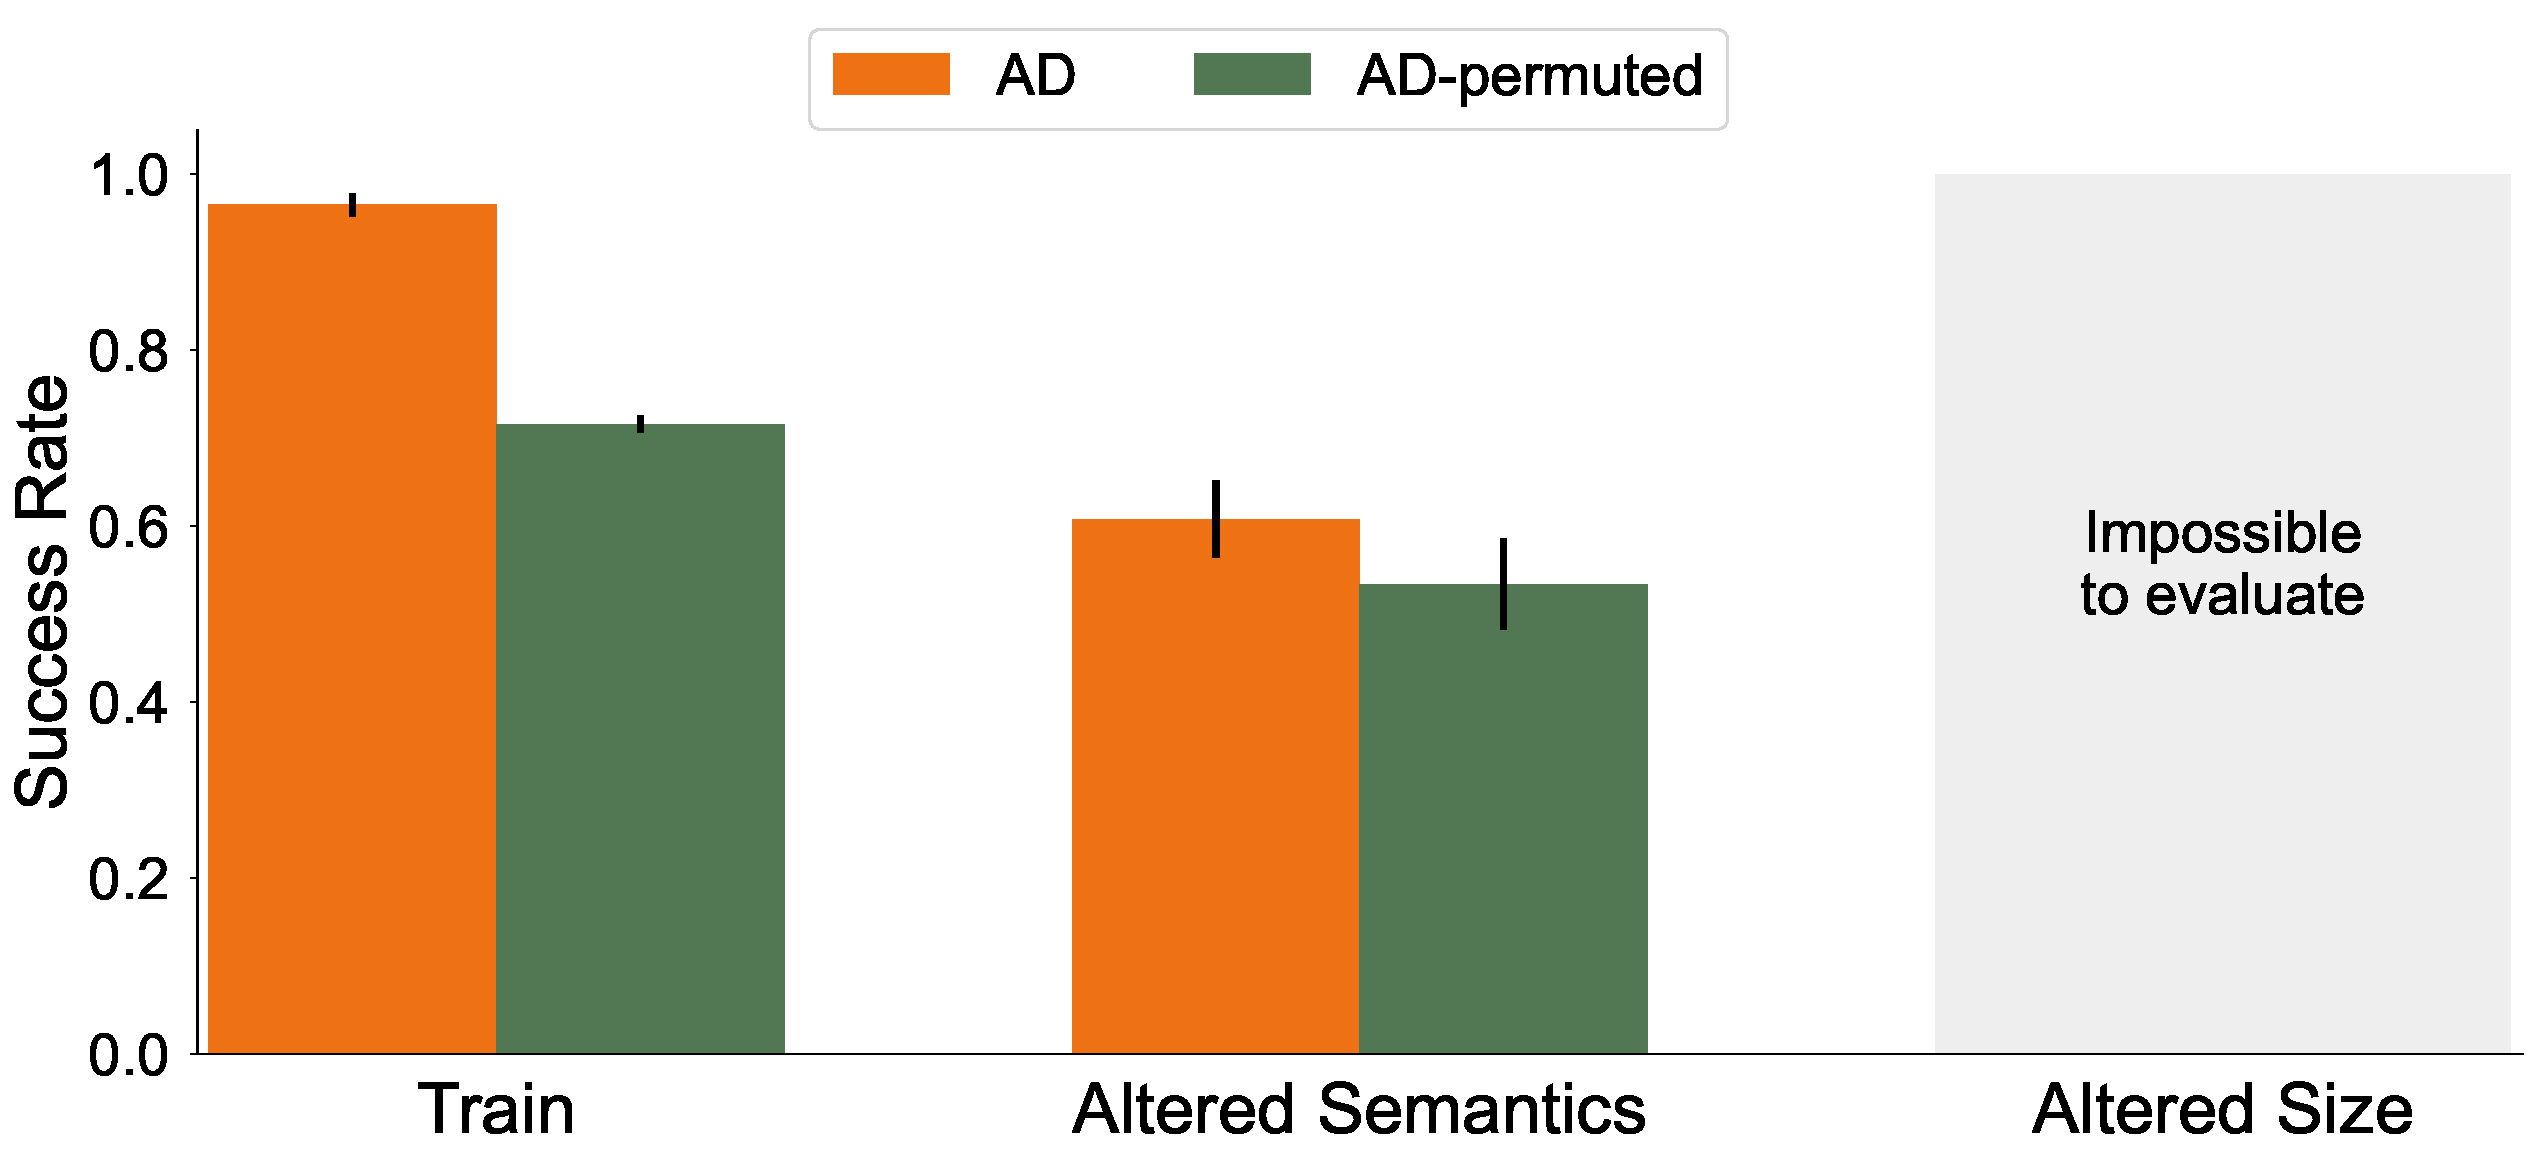
\includegraphics[width=\columnwidth]{images/bad_ad.pdf}
    % 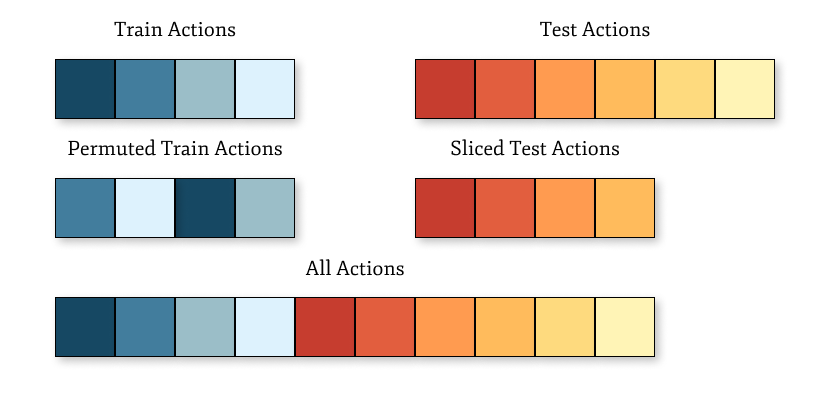
\includegraphics[width=\columnwidth]{visualizations/action_sets_vis_2.png}
    \caption{\textbf{Algorithm Distillation Struggles with Novel Action Spaces:} Despite its good results on the train action set, AD's performance diminishes when the action semantics change, either due to a permutation or substitution. It is important to note that augmenting the training data with permuted action sets does not lead to increased performance, signifying that action set invariance should be enforced from a model design standpoint. Additionally, it is impossible to apply a trained AD model to a larger action set. On the graph, the bars are the success rate values on the Darkroom environment (described in \Cref{sec:exp_gridworld}) obtained after evaluating each of the action sets visualized in \Cref{fig:action_sets_viz}, averaged over 5 runs. \textit{Altered Semantics} aggregate the values from the \textit{Permuted Train Actions} and \textit{Sliced Test Actions} sets. \textit{Altered Size} aggregates the values from \textit{Test Actions} and \textit{All Actions}. See \cref{sec:exp_gridworld} for more information about the construction of the action sets.}
    \label{fig:bad_ad}
    \vskip -0.2in
\end{figure}



\begin{figure}[t]
    \vskip 0.2in
    \centering
    % \includegraphics[width=0.95\textwidth]{images/new_regrets.pdf}
    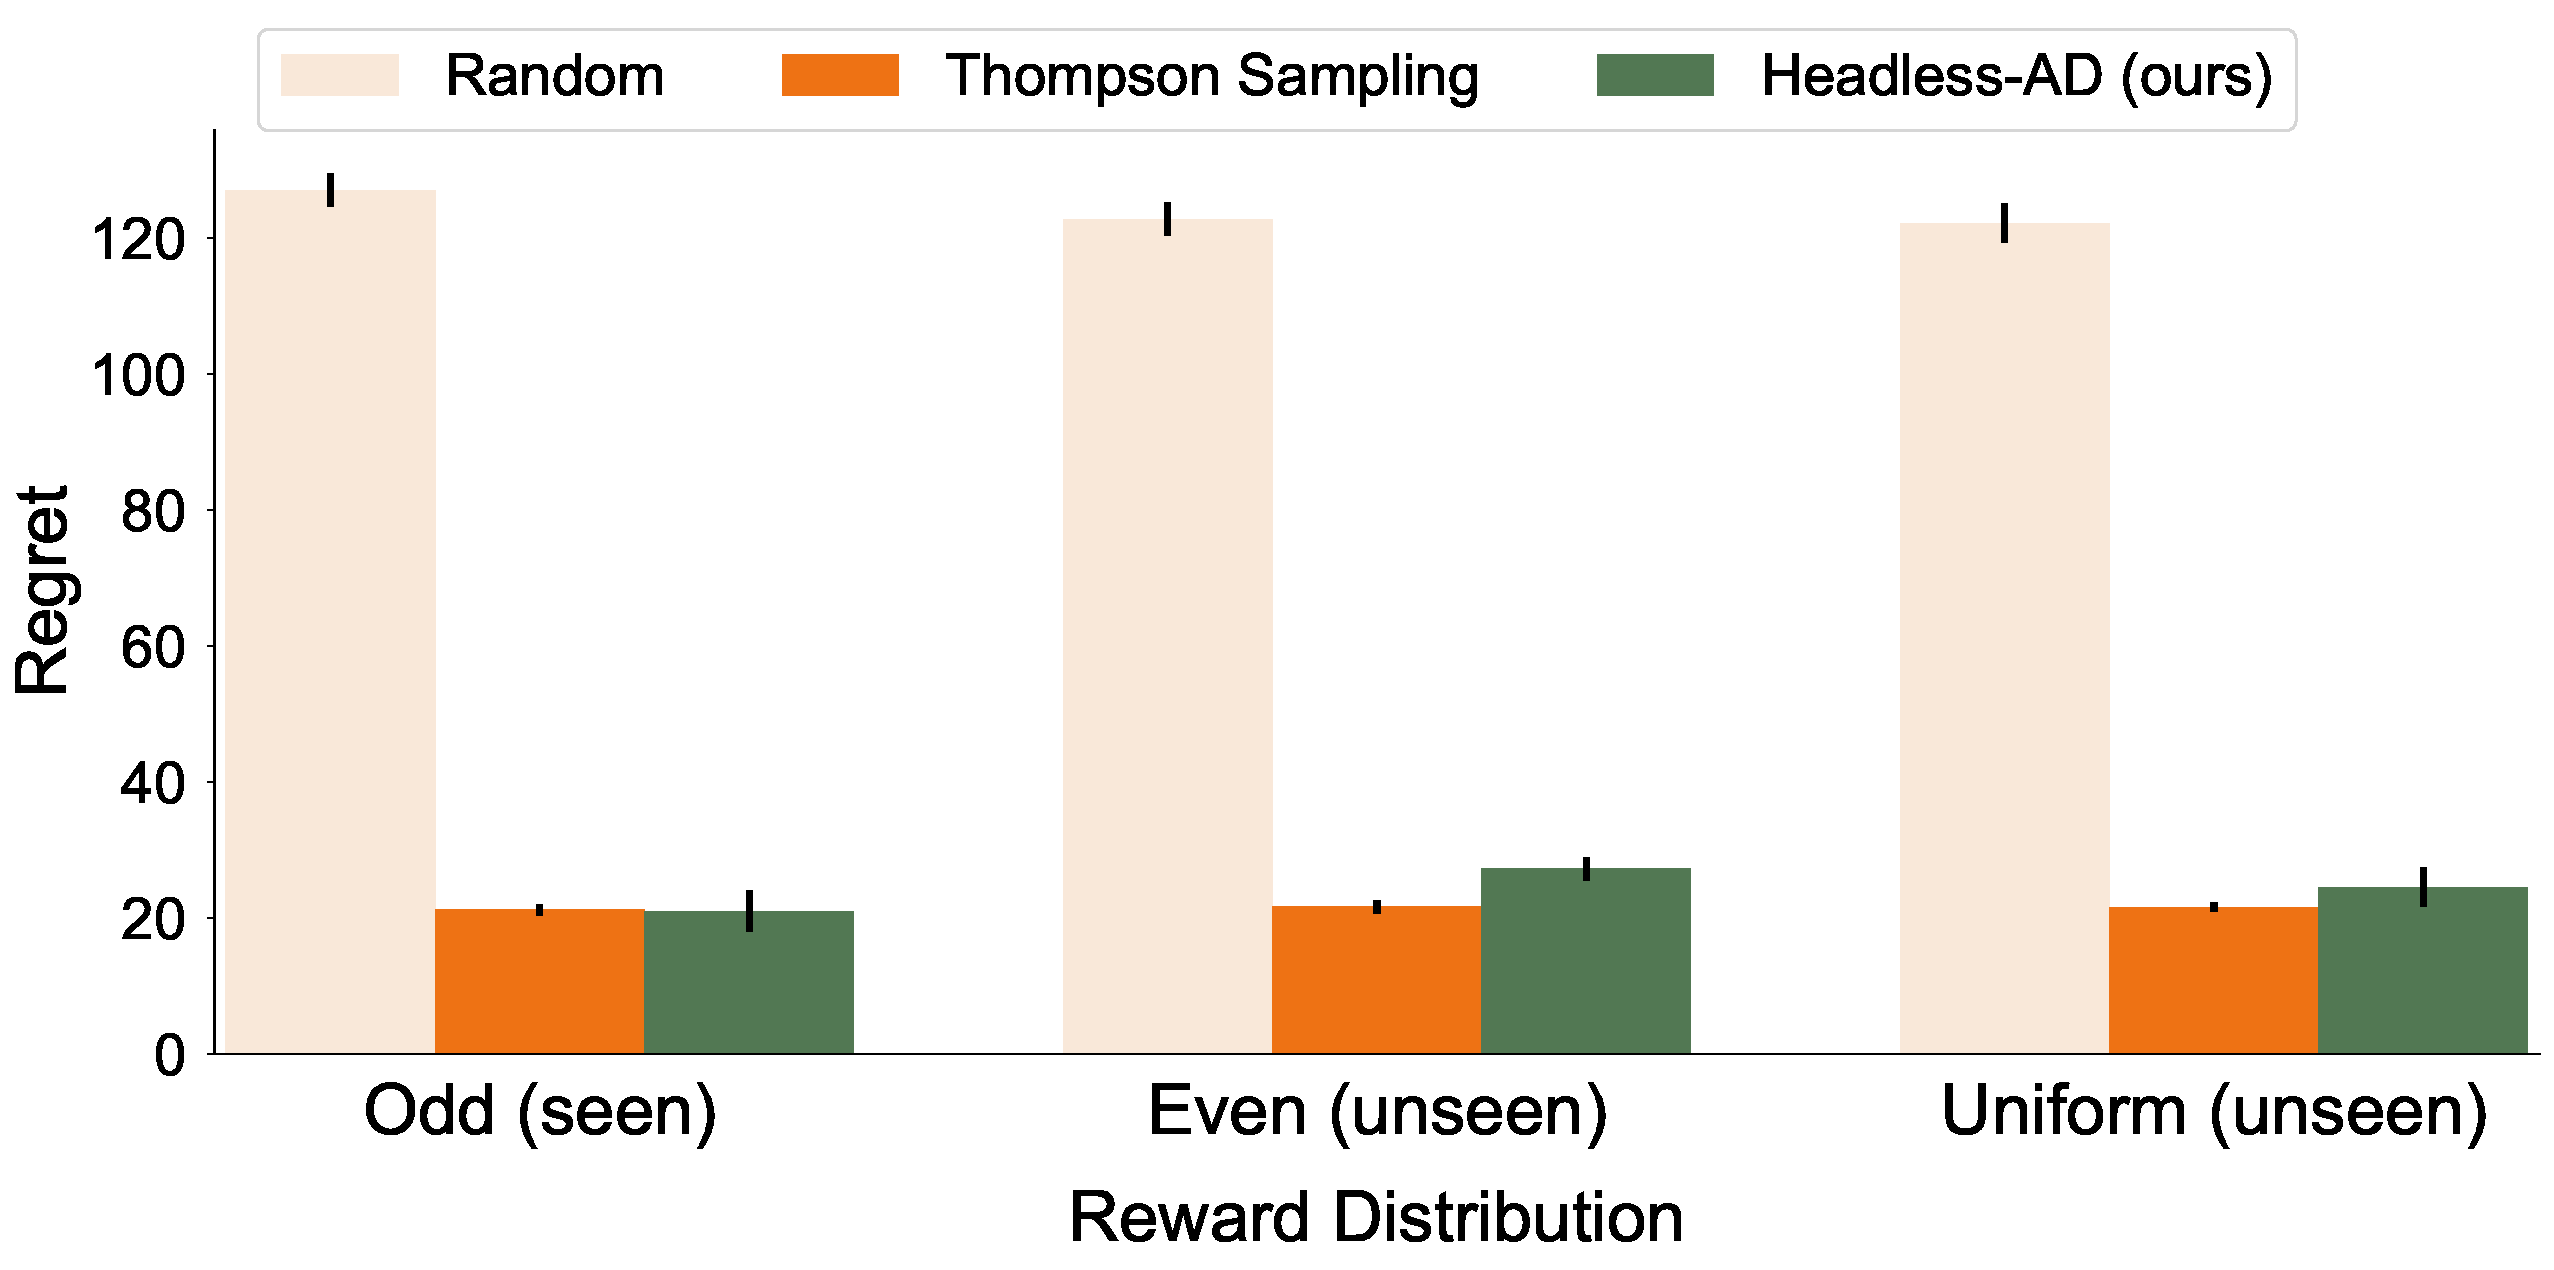
\includegraphics[width=\columnwidth]{images/bandit_new_regrets.pdf}
    \caption{\textbf{Algorithm Regret under Variable Reward Distributions in Bernoulli Bandit:} The graph compares regret for Random, Thompson Sampling, and Headless-AD across distinct reward distributions in the Bernoulli Bandit environment, averaged from five seeds. During training, the high reward was $95\%$ more likely to distribute across the odd arms. During testing, it either switched to the even arms or a uniform distribution. Note that Headless-AD maintains high performance in all configurations, proving its ICL capabilities at generalizing to novel tasks, represented by changes in reward distribution. Data is aggregated from bandit problems with $4-20$ arms, reflecting the training conditions.}
    \label{fig:bandit_new_regrets}
    \vskip -0.2in
\end{figure}

To mitigate the action space limitations of AD, we propose Headless-AD, a new architecture that improves on AD by omitting the final linear layer and incorporating three key modifications. The Headless-AD architecture and data flow are visualized in \Cref{fig:model_vis}.

% \textbf{Random Action Embedding Strategy:} To prepare the model for potential new actions during testing, we transition from static learned action embeddings to dynamic embeddings generated by a mapping function $g:~\mathbb{A}~\rightarrow~\mathbb{R}^n$, which produces a unique random encoding for each action in a batch at the start of every training step. The mapping is shared across all batch instances and is consistent along the context sequence, i.e., actions with index $i$ in their respective action sets will all be mapped to the same embedding. The random embeddings are constrained as orthogonal vectors within a unit sphere. The details of the sampling process can be found in \Cref{appendix:orthonormal_vectors}. This approach makes the model deduce action semantics from the interaction history. The orthogonality also clarifies the interpretation of similarity measures as logits because it isolates the similarity of each action, thus preventing overlap in the probability distribution. Moreover, employing random embeddings enhances data variety, which has been demonstrated to boost in-context learning for RL agents \citep{kirsch2023towards, lu2023structured}.

\textbf{Random Action Embeddings:} To remove the dependence of the model on the pretrained action embeddings, we employed a dynamic mapping function $g:~\mathbb{A}~\rightarrow~\mathbb{R}^n$, which produces a unique random encoding for each action in a batch at the start of every training step. The mapping is shared across all batch instances and is consistent along the context sequence, i.e., actions with index $i$ in their respective action sets will all be mapped to the same embedding. During inference, we generated a single set of embeddings at the beginning and used them throughout the evaluation.

The core intuition behind employing random action embeddings is to eliminate any prior knowledge about the structure of the action space within our model. This approach stems from our observation that using learnable embeddings for actions becomes impractical when encountering new actions not seen during training. A new action would lack a pre-trained embedding, and assigning an arbitrary embedding could introduce an undesirable domain shift, as the model would not recognize it. Moreover, allowing the model to learn new embeddings on-the-fly would necessitate extra gradient steps, diverging from our goal of maintaining a zero-shot learning framework. The usage of random action embeddings ensures that the model does not depend on extracting any information from the embeddings themselves but rather relies on interpreting the context provided by historical interactions with the environment. Moreover, employing random embeddings enhances data variety, which has been demonstrated to boost in-context learning for RL agents \citep{kirsch2023towards, lu2023structured}.


\begin{figure*}[t]
    \vskip 0.2in
    \centering
    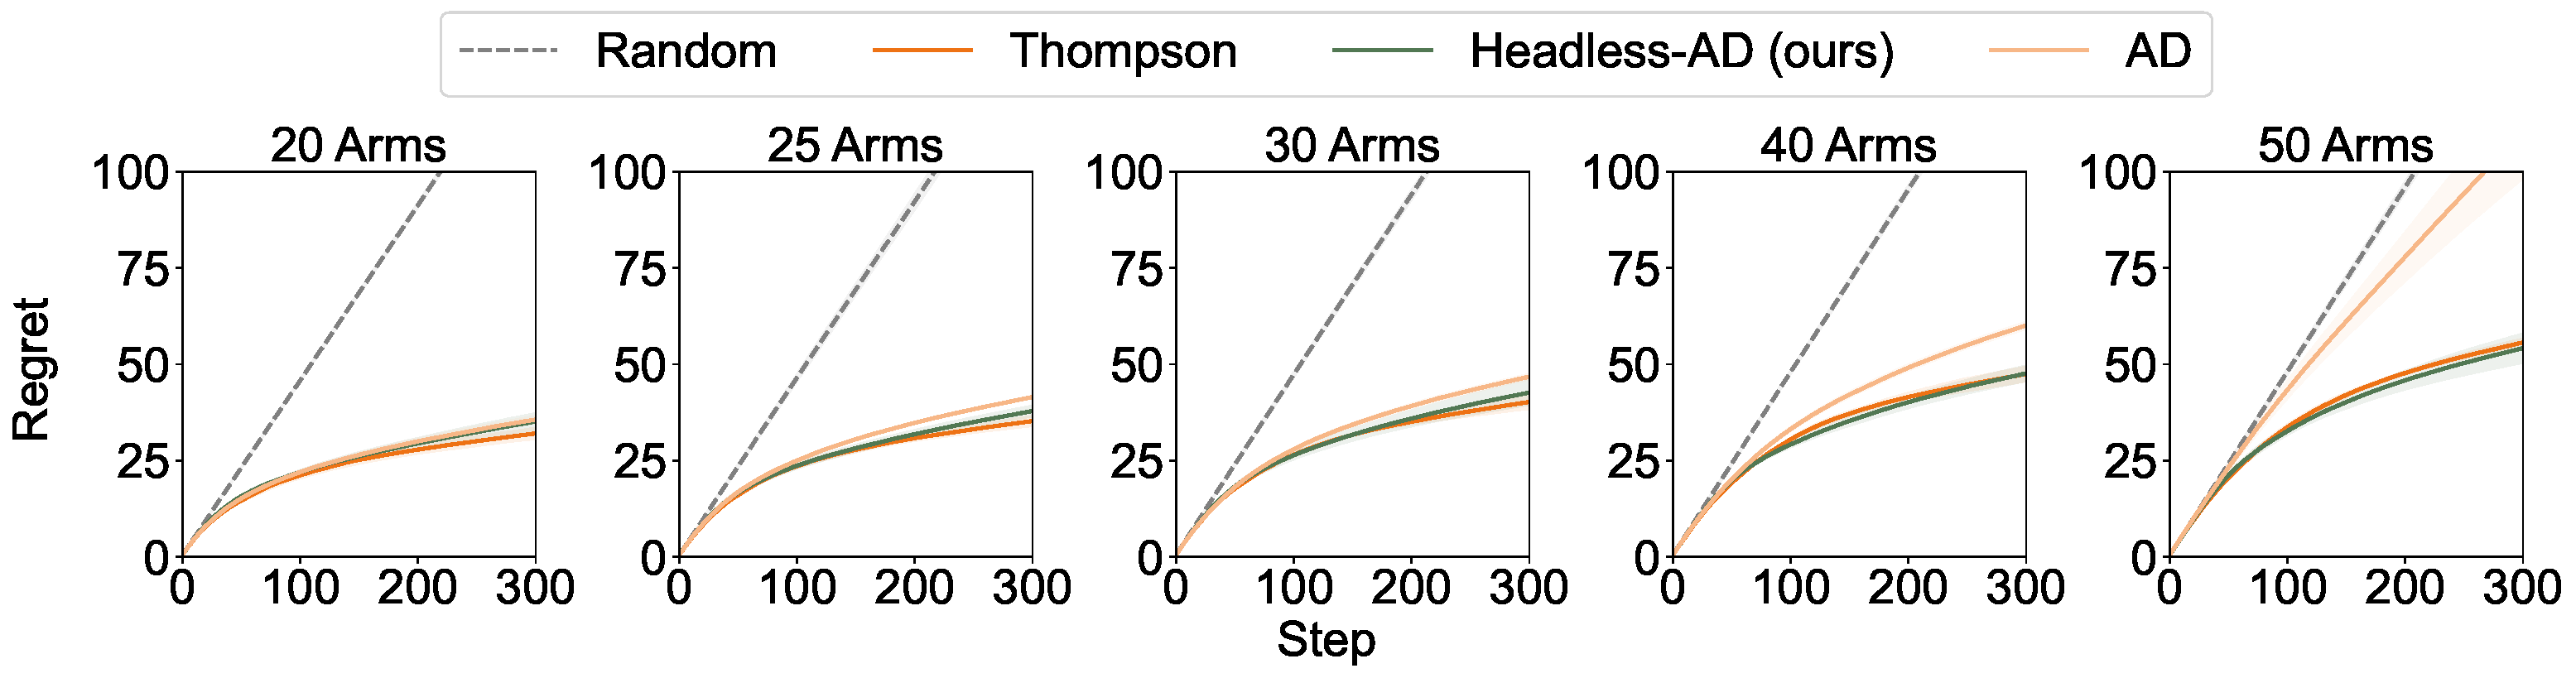
\includegraphics[width=0.95\textwidth]{images/bandit_together.pdf}
    \caption{\textbf{Algorithm Regret under Increasing Amount of Arms in Bernoulli Bandit:} This series of plots shows the regret of Thompson Sampling, AD, and Headless-AD algorithms over evaluation steps in environments with $20-50$ arms, averaged from five seeds with $100$ bandits each. Although Headless-AD has been trained on bandits with up to $20$ arms, it performs well, matching or outperforming other algorithms in larger arm settings without additional training. Note that AD was retrained from scratch for each task with a different number of arms.}
    \label{fig:bandit_together_curves}
    \vskip -0.2in
\end{figure*}


We further refined this strategy by constraining the random embeddings to lie on a unit sphere and ensuring their orthogonality (see \Cref{appendix:orthonormal_vectors}). The choice of a unit sphere normalizes the scale of the embeddings, while orthogonality allows the model to independently adjust the probability assigned to each action. This condition is crucial for preventing unintended probability mass allocation to multiple actions when the model's prediction vector aligns with one embedding vector. A similar concept is explored by \citep{elhage2022superposition} in the context of feature interference.

\textbf{Direct Prediction of Action Embeddings:} The model output is modified to yield an action embedding $\hat{a}^{emb}_t$ rather than a probability distribution over actions. This alteration makes the model independent of action set size and order, granting it permutation invariance. The InfoNCE Contrastive Loss \citep{oord2018representation}, diverging from its usual role in representation learning \citep{jaiswal2020survey}, serves as a regression objective to reinforce the similarity between the model prediction and the subsequent action in the data. All other actions are treated as negative samples. Thus, the objective is 
\[
L = -\mathop{\mathbb{E}}\left[{\log{\frac{e^{f(\hat{a}^{emb}_t, a^{emb}_t) / \tau}}{\sum_{a \in A}{e^{f(\hat{a}^{emb}_t, a^{emb}) / \tau}}}}}\right],
\]
where $a^{emb} = g(a)$ and $\tau$ is a temperature parameter. We used dot-product as the similarity function $f$. 

\textbf{Action Set Prompt:} To address the model's lack of awareness of the action space structure caused by the two previous changes, we prepend the input with a sequence of embeddings for all available actions.

The modified input format is thus represented as
\[
h_t = \left(a^{emb,0}, \dots, a^{emb,N}, o_{<t}, a^{emb}_{<t}, r_{<t}, o_t\right),
\]
where $N$ is the action set size. An illustrative code snippet with Headless-AD's training procedure can be found in \Cref{appendix:pseudo_code}.
\newline
\newline
% 'suggest' instead of 'employ'
We suggest two methods to select actions during inference: (1) nearest neighbor selection:
\[
a = \arg \max_{a \in A} f(\hat{a}^{emb}, a^{emb})
\]
and (2) probabilistic sampling based on the similarity to the predicted action embedding:
\[
P(a_i) = \frac{e^{f(\hat{a}^{emb}, a^{emb}_i)}}{\sum_{a \in A}{e^{f(\hat{a}^{emb}, a^{emb}}})}.
\]
We treat the specific choice of method as a hyperparameter.